\section{The problem}\label{sec:problem}

\evlit{} Practice compiles a sequence of decisions into a fast, automatic procedure that no longer
needs the knowledge it was built from \parencite{anderson1982acquisition}. Its steps become
\enquote{not available for introspection} \parencite[p.~584]{clark2008cognitive}. An expert who
explains a familiar task therefore omits steps, not out of reticence, but because they no longer
come to mind. How much any one report leaves out is an empirical question.

\subsection{What omission looks like when it is measured}

\begin{evlitbox}
  Three surgeons, videotaped teaching a cricothyrotomy, were compared against a 46-step task list
  built by CTA from three other surgeons. On average they omitted 71\% of clinical-knowledge steps
  (10 of 14), 51\% of action steps (14 of 27) and 73\% of decision steps (3.6 of 5), and described
  \emph{how} to perform only 13\% of action steps. Directed CTA prompting raised the share of steps
  each surgeon described from 44\% (20 of 46) to 66\% (31 of 46) \parencite{sullivan2014use}.
\end{evlitbox}

\evlit{} Two other studies give numbers. Six expert programmers explained their troubleshooting
under several elicitation methods \parencite{chao1994percentage}. As reported by
\textcite[p.~585]{clark2008cognitive} (we did not check the original tables), no single expert reported
more than 41\% of diagnostic actions, 53\% of debugging actions or 29\% of interpretations; pooling all
six raised coverage to 87\%, 88\% and 62\%.
Critical Decision Method (CDM) interviews with neonatal intensive-care nurses produced a
sepsis-assessment guide with information \enquote{not available in the current literature}
\parencite{crandall1993critical}.

\evint{} These studies do not license a single omission rate. Each has 3 to 17 experts in one domain,
and their gold standards are themselves built by CTA. The figure often quoted outside this
literature, that experts are unaware of about 70\% of their own decisions, is not a new measurement;
\textcite[p.~591]{clark2008cognitive} state it citing earlier reviews. We treat the direction as
established: experts omit a large, variable share of decisions, cues and interpretations.

\begin{figure}[tbp]
  \centering
  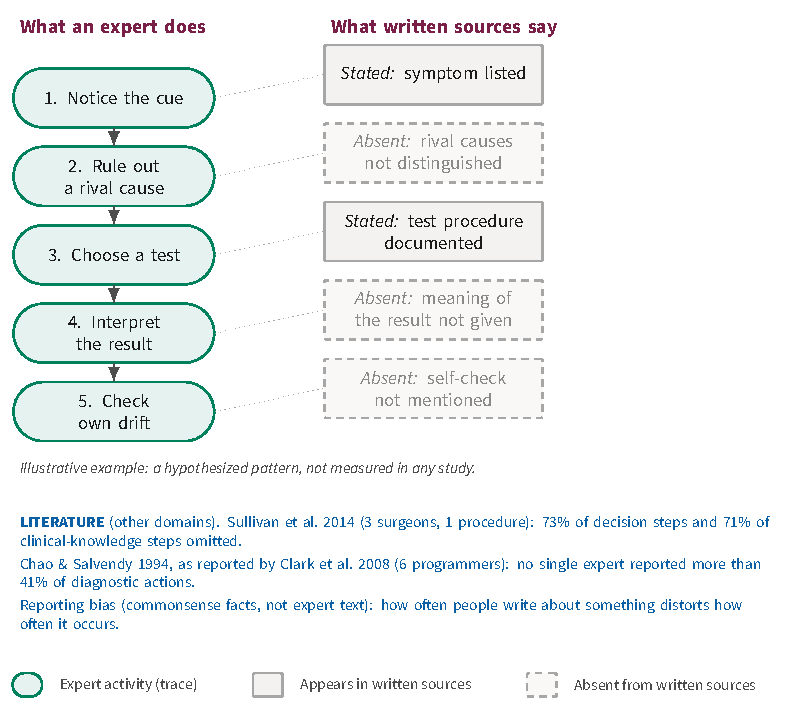
\includegraphics{figures/pdf/fig01_problem.pdf}
  \caption[What reaches text, and what does not]{What part of expert knowledge reaches text, and
    what does not. The task trace is illustrative, not measured. Automaticity and measured omission in
    three small studies show that experts' own reports leave out many decisions, cues and
    interpretations; reporting bias is shown for commonsense facts. That written expert sources omit
    the same kinds of knowledge is our hypothesis, not a finding of these studies.}
  \label{fig:problem}
\end{figure}

\subsection{Writers omit the obvious too}

\evlit{} How often people write about actions, outcomes and properties systematically distorts how
often they occur \parencite{gordon2013reporting}. Text-only language models inherit the distortion,
for example in the colors they predict for 521 objects \parencite{paik2021world}. Both studies concern
commonsense facts, not expert documentation. \evhyp{} We transfer the idea: omission in speech and
reporting bias in text may point at the same target in expert sources, namely cues, decisions,
interpretations, checks and the boundaries of hedged rules. This transfer is untested. AI can make the boundary between what is written and what is not sharper and more
auditable; it cannot tell on its own whether a silence hides expert knowledge, an unrecorded fact, or
nothing. That needs a human answer (\cref{fig:problem}).

\subsection{One education and one organizational example}

\evlit{} \emph{Education.} Experts sort physics problems by the principle that solves them; novices
sort them by surface features \parencite{chi1981categorization}. For the expert, choosing the
principle happens as recognition, not as a step, so it goes unsaid. Experts are also unreliable
judges of what learners find hard: 25 physics teaching assistants and 30 instructors predicted
students' most common wrong answers at 65\% and 68\% of the maximum score, against 40\% for random
guessing, with no difference between the groups \parencite{maries2016teaching}. Hence expert or AI guesses about
learner difficulty are never treated as evidence here.

\evlit{} \emph{Organizations.} Photocopier technicians diagnose through shared stories of how a
machine actually fails; those stories, not the service manual, keep the group's knowledge current
\parencite{orr1996talking,brown1991organizational}. \evobs{} On public PLC troubleshooting text, the
gap map produced a record of the same shape from the span \enquote{a common mistake\dots\ is
panicking and abandoning systematic approaches}: the sources name the failure mode, and the absence
check found at most a partial statement of how a troubleshooter notices the drift into
it.\footnote{\repo{research/n3/plc/gapmap.json}, the GUARD-lens record at rank~9.} This shows only
that a lens can flag text of this \emph{shape}.

\evlit{} \emph{Why it matters.} In a study of best-practice transfer inside firms, the major barriers
were knowledge-related (the recipient's lack of absorptive capacity, causal ambiguity, and an arduous
relationship between source and recipient) rather than mainly motivational
\parencite{szulanski1996exploring}. Many popular open-source projects depend on one or two developers
\parencite{avelino2016novel}, and turnover exposes projects to knowledge losses far above the expected
loss \parencite{rigby2016quantifying}. \evint{} Training, onboarding and succession can suffer when such
knowledge is not made explicit before its holder leaves.
